\section{\acl{WSDE}}
\label{sec:04_tdoaSingle}

Before evaluating the performance of the different methods as a whole,
% For comparability of the results,
one exemplary measurement is utilized
to present and analyse the \ac{TDOA} methods in detail first.
In this recording, the sound source is placed at the right front
of the robot with 4.5\si{m} distance.
Hereinafter, this measurement will be referenced to as \textit{demonstration-dataset}.
This corresponds to an an angle of -33.7\si{\degree} in robot coordinates.
To get an idea about the examined data, according whistle signal samples around the
start are plotted in \cref{fig:04_tdoaSignal} for all channels.
% -------------------------------------------------------------
\begin{figure}[ht]
	\centering
	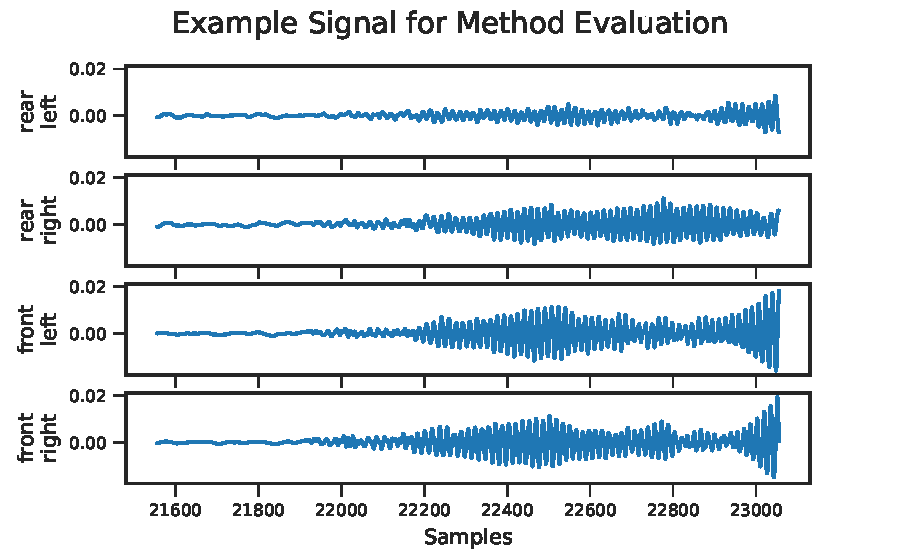
\includegraphics[]{figures/evaluation/cc_frontRight_1_signal}
	\caption{Signal start section of a whistle-sound recorded from front right.}
	\label{fig:04_tdoaSignal}
\end{figure}
% -------------------------------------------------------------

As the next sections focus on the performance of the \ac{TDOA} methods,
the start index is set manually.

For the sake of conciseness, throughout the following sections the correlation
function $R_{x_ax_b}$ of two signals $x_a$ and $x_b$  (\cf
\cref{chap:02_prerequisites}) is denoted as $R_{ab}$.


\subsection{Cross Correlation}
\label{subsec:04_ccSingle}
% -------------------------------------------------------------

The \ac{CC} is a widespread technique to obtain the time delay
between two series of samples.
To discuss the result of the \ac{CC}, the belonging correlation functions
of the demonstration-dataset are plotted in \cref{fig:04_cc}.
The selection process and implementation correspond to the explanations
in \cref{subsubsec:03_cc}.
For $R_{32}$ and $R_{13}$ a peak is clearly visible.
However, for the other \ac{CC} the problem of a weak peak
arises what was mentioned as downside of the \ac{CC} in \cref{sec:02_cc}.
% -------------------------------------------------------------
\begin{figure}[ht]
	\centering
	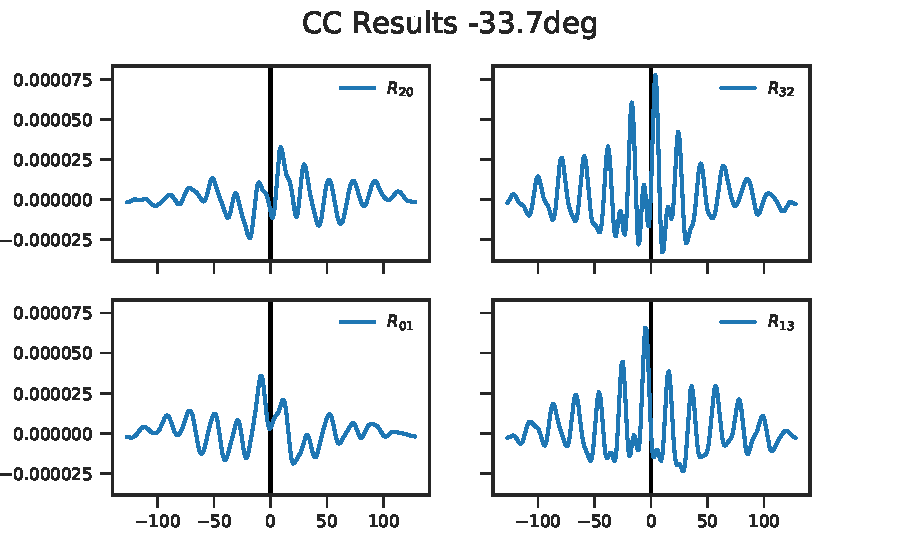
\includegraphics[]{figures/evaluation/cc_frontRight_1}
	\caption{Cross correlation results of signal from front right (-33.7\si{\degree}).}
	\label{fig:04_cc}
\end{figure}
% -------------------------------------------------------------
\btline{ht}{1.2}
\btab{|c|c|c|c|c|}
\hline
Base Channel & Next Channel & Delay & Candidate (-) & Candidate (+)\\
\hline
0 & 1 & -8.25 & -144.9 & -35.1\\
\hline
1 & 3 & -4.59 & -17.4 & 78.6\\
\hline
2 & 0 & 9.16 & -30.6 & -30.6\\
\hline
3 & 2 & 3.94 & -150.2 & -29.8\\
\hline
\etab
\et{Cross correlation delay results of signal from front right}{04_cc}
% -------------------------------------------------------------

According to the delays in \cref{tab:04_cc}, two source direction candidates arise
for each channel pair.
By the implementation in \cref{subsec:03_directionCandidates}, the combination of
all options with the smallest error is selected as \ac{WSDE}.
Hence, the algorithm outputs -26.9\si{\degree} what produces an error of 6.8\si{\degree}.
The delay between channel 2 and 0 is larger than the maximum delay of 6.85 samples
and therefore cut to the maximum sample delay.
Besides these, the \ac{TDOA} between the channel pairs produce one appropriate
direction candidate which correctly points to the sound source.
% -------------------------------------------------------------

\subsection{Generalized Cross Correlation}
\label{subsec:04_gccSingle}
% -------------------------------------------------------------
\Cref{fig:04_gcc} presents the \ac{GCC} result by the \ac{GCC-PHAT} method of
the demonstration-dataset equal to \cref{subsec:04_ccSingle}.
The subsample delays for each channel pair and their resulting direction candidates
are listed in \cref{tab:04_gcc}.
From this, a final direction of -30.0\si{\degree} is determined
resulting in an error of 3.69\si{\degree}.
It is apparent that the peaks of the \ac{GCC} are better to detect than the peaks of the
\ac{CC}.
% -------------------------------------------------------------
\begin{figure}[ht]
	\centering
	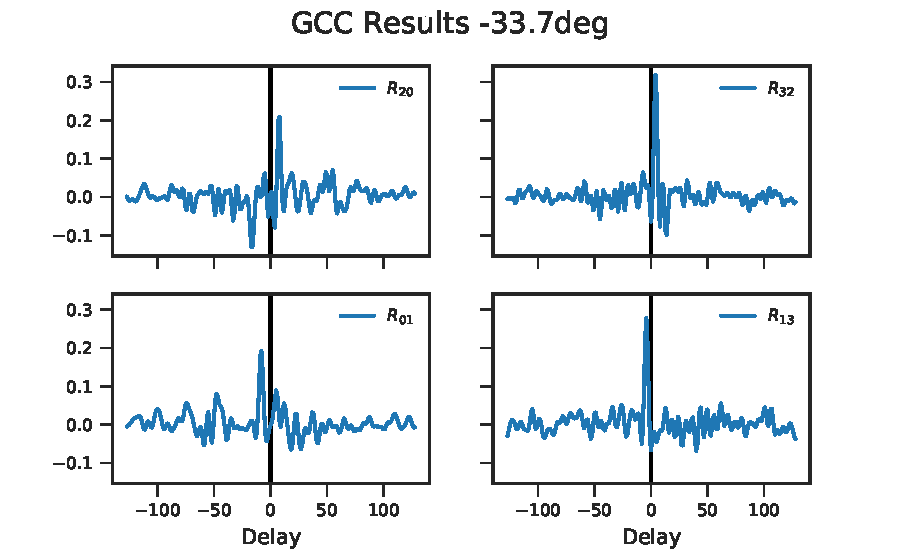
\includegraphics[]{figures/evaluation/gcc_frontRight}
	\caption{Generalized cross correlation results of signal from front right.}
	\label{fig:04_gcc}
\end{figure}
% -------------------------------------------------------------
\btline{ht}{1.2}
\btab{|c|c|c|c|c|}
\hline
Base Channel & Next Channel & Delay & Candidate (-) & Candidate (+)\\
\hline
0 & 1 & -8.28 & -144.7 & -35.3\\
\hline
1 & 3 & -4.09 & -22.8 & 84.0\\
\hline
2 & 0 & 7.60 & -30.6 & -30.6\\
\hline
3 & 2 & 4.13 & -148.7 & -31.3\\
\hline
\etab
\et{Generalized cross correlation delay results of signal from front right}{04_gcc}
% -------------------------------------------------------------
\subsection{Phase Difference}
\label{subsec:04_phaseSingle}

For detecting the source direction with phase difference, a smaller frame
size of 64 samples is defined.
In \cref{subsubsec:03_phase} two variants of this method were introduced that use
different strategies to identify a reference frequency. The first version uses
a static reference frequency that is fixed a-priori by the user. The second version
dynamically estimates a dominant frequency across all four channels. Hereafter,
the performance of both variants is discussed.


\subsubsection*{Static Reference Frequency}

In \cref{subsubsec:03_phase} two different ways to set a reference frequency $f_c$
for the phase difference method were introduced.
First, a suitable value for the reference frequency is specified by
examining the influence of the chosen value.
Therefore, \ac{WSDE} results with the phase difference method are evaluated by setting
different values for the reference frequency within whistle range.
For this purpose we consider all of eleven measurements of the the laboratory-dataset
recorded with robot no. 26 at the center point.

According to \cref{subsubsec:03_phase}, the most feasible frequency is defined as
2775.08\si{\hertz} by the distance between the channels
and the whistle spectrum ranges between 2\si{\kilo\hertz}
and 4\si{\kilo\hertz}.

As shown in \cref{fig:04_diffFc} shows, the \ac{RMSE} is high for
frequencies smaller than 2600\si{\hertz}.
With a frequency of 2024.12\si{\hertz}, error is largest.
% The result complies with the information in \cref{fig:03_maxFreq} showing that
% frequencies higher than 2500\si{\hertz} are dominant in whistle signals.
With this outcome, the fixed frequency is set to 2670.1\si{\hertz}
for further usage of the direction detection by phase method.
Limitation exists due to the ambiguity of the signal which is
content of \cref{subsubsec:03_phase}.
% -------------------------------------------------------------
\begin{figure}[ht]
	\centering
	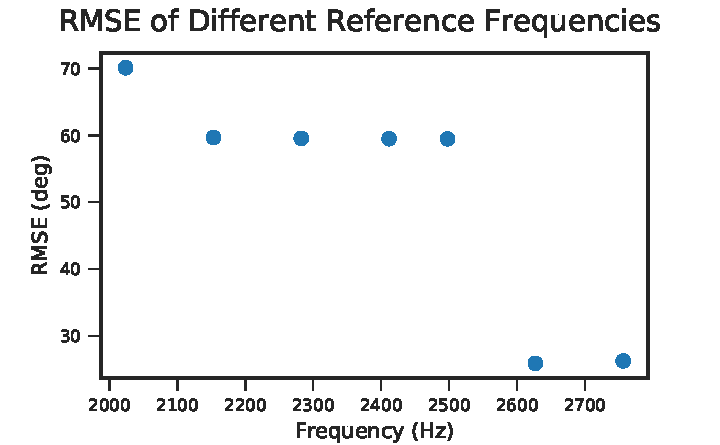
\includegraphics[]{figures/evaluation/phase_fc_rmse}
	\caption{Result of all measurements done with robot 26 to compare different
		fixed frequency values in whistle range.}
	\label{fig:04_diffFc}
\end{figure}
% -------------------------------------------------------------

On the basis of the results, the reference frequency was set to a minimum
of 2600\si{\hertz} for evaluation of the demonstration-dataset.
Hence, the reference frequency is 2627.1\si{\hertz} in the case of a \ac{FFT} length
of 256 samples.
Applying the phase difference method with this reference frequency, the final
direction estimate computed from the candidates listed in
\cref{tab:04_fixedFreqResult} is -29.6\si{\degree} which results in an error of
4.1\si{\degree}.
% -------------------------------------------------------------
\btline{ht}{1.2}
\btab{|c|c|c|c|c|}
\hline
Base Channel & Next Channel & Phase Difference & Candidate (-) & Candidate (+)\\
& & [\si{\deg}] & [\si{\deg}] & [\si{\deg}] \\
\hline
1 & 3 & -79.1 & -26.8 & 88.0\\
\hline
2 & 0 & 167.7 & -30.6 & -30.6\\
\hline
3 & 2 & 88.5 & -148.7 & -31.3\\
\hline
\etab
\et{Resulting candidates of phase difference method with fixed frequency
	2670.1Hz of example measurement from front right
	(-33.7\si{\degree})}{04_fixedFreqResult}
% -------------------------------------------------------------

\subsubsection*{Dynamic Reference Frequency Selection}

Another option is to have a nonspecific reference frequency that
is computed dynamically without a-priori knowledge.
As stated in the implementation chapter, frames are chosen where the frequencies
of the maximum amplitudes coincides for all channels.
For the running example discussed here, this corresponds to a frequency of 2756.25\si{\hertz}.

For comprehensibility, the determined frequency information visualized by
wave signals with the detected phases and amplitudes
in the lower subplot of \cref{fig:04_phaseSingle}.
In the upper plot of \cref{fig:04_phaseSingle} one sees the originally received microphone
data before applying a Hann window and transforming it into frequency domain by
\ac{FFT}. The resulting phases and amplitudes are listed in
\cref{tab:04_phaseSingle}.
% -------------------------------------------------------------
\begin{figure}[h]
	\centering
	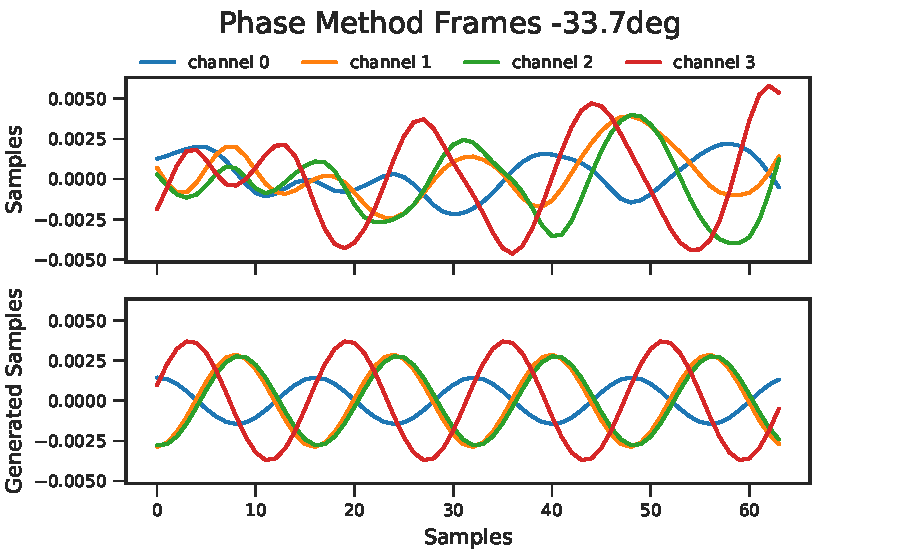
\includegraphics[]{figures/evaluation/phase_cos}
	\caption{Frames used for the direction detection by phase method.}
	\label{fig:04_phaseSingle}
\end{figure}
% -------------------------------------------------------------
\Cref{tab:03_maxFrequencies} pointed out that the most feasible frequency
of the rear channels 0 and 1 is not in whistle spectrum
due to the larger physical distance between the microphones.
Thus, the phase difference information is neglected because of the ambiguity of
the temporal sequence between the signals.
Following the procedure discussed in \cref{subsubsec:03_phase},
the resulting phase difference estimate
is -29.2\si{\degree} by combining the candidate direction -17.6\si{\degree},
-30.6\si{\degree} and -39.3\si{\degree} from channels 1, 2 and 3 according to
\cref{tab:04_phaseDiffSingle}.
% -------------------------------------------------------------
\btline{ht}{1.2}
\btab{|c|c|c|}
\hline
Channel & Phase [\si{\deg}] & Amplitude\\
\hline
0 & -1.55 & 0.00144\\
\hline
1 & -177.7 & 0.00287\\
\hline
2 & 173.4 & 0.00279\\
\hline
3 & -75.0 & 0.00372\\
\hline
\etab
\et{Phase and amplitude of frame signals with $f_c$ = 2756.25Hz}{04_phaseSingle}
% -------------------------------------------------------------
\btline{ht}{1.2}
\btab{|c|c|c|c|c|}
\hline
Base Channel & Next Channel & Phase Difference & Candidate (-) & Candidate (+)\\
& & [\si{\deg}] & [\si{\deg}] & [\si{\deg}] \\
\hline
1 & 3 & -102.7 & -17.6 & 78.8\\
\hline
2 & 0 & 173.4 & -30.6 & -30.6\\
\hline
3 & 2 & 113.1 & -140.7 & -39.3\\
\hline
\etab
\et{Phase differences and resulting direction candidates of demonstration-dataset
	with dynamically determined reference frequency}
{04_phaseDiffSingle}
% -------------------------------------------------------------

\subsubsection*{Impact of Selected Frame}
\label{subsubsec:04_frameNumber}

Not only does the frequency play a major role for the phase method,
but also the samples chosen for analysis.
Again it is referred to the eleven measurements of the laboratory-dataset
recorded on the robot at the center point (no. 26).
To evaluate if and how the result changes over time, the selection window
is shifted by half the frame size from -5 shift steps to 20.
Recapitulating the implementation details for the static reference frequency case
in \cref{subsec:04_phaseSingle},
the first frame after the start index is chosen in which the whistle detection would
count a whistle signal.
This frame is represented by zero shift.

% [ 62.32629763  59.19634105  66.78950798  54.53898736  30.80692207
%   25.91537359  56.55427899  65.27548831  66.3898905   75.48670644
%   97.33965933  96.6373387  100.22012166 104.20160752  59.55737843
%   58.22148221  48.51237213  51.93254436  49.08273252  62.64453085
%   56.49506079  57.03430393  67.46509351  73.21671739  43.69704948]
In \cref{fig:04_phaseOverTime}, the resulting errors per shift
for all measurements are plotted, presenting the influence of the
selected frame around the signal start.
The reference frequency was set to 2627.1\si{\hertz} due to the
outcome that frequencies larger than 2600\si{\hertz} achieve best results.
The graph presents that frames nearest to the signal start reach best results
with an \ac{RMSE} of 25.9\si{\degree}.
These results show that the frame position has a significant influence on the prediction
accuracy of the direction detection.
Therefore, an accurate signal start detection is crucial for the preciseness of the \ac{SSL}
by phase difference.
% -------------------------------------------------------------
\begin{figure}[ht]
	\centering
	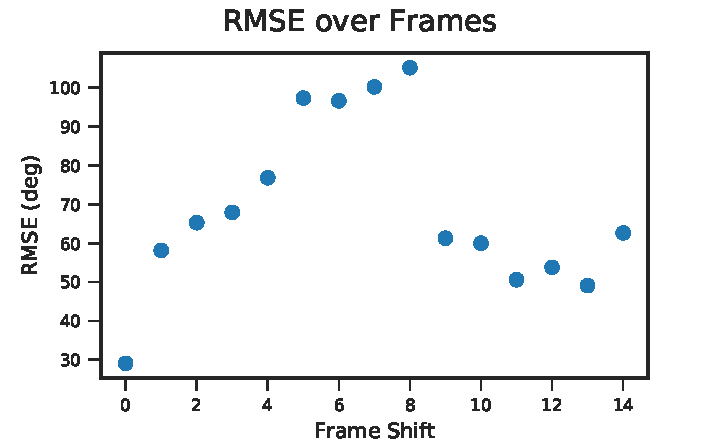
\includegraphics[]{figures/evaluation/phase_over_time}
	\caption{\ac{WSDE} result errors while shifting the frame over the
		samples of the laboratory-dataset on robot no 26.}
	\label{fig:04_phaseOverTime}
\end{figure}
% -------------------------------------------------------------

\subsubsection*{Phase Method Conclusion}
\label{subsubsec:04_phaseMethodConclusion}

Different options were investigated relating to the phase difference method
in the last subsections.
One finding is that reference frequency values should be chosen larger than
2.6\si{\kilo\hertz} for best results.
Another is that samples at the beginning of the signal are most suitable
for this method.
An advantage of the dynamically selected reference frequency is the reduction of
one parameter.
It requires more effort to implement and considering edge cases but
does not depend on the whistle detection.
Both approaches are valid for this work and result in a similar reference
frequency due to the limitations listed in \cref{subsubsec:03_phase}.

\subsection{\ac{TDOA} Method Comparison}
\label{subsec:04_singleRobotAngleError}

As the different \ac{TDOA} methods were discussed profoundly in the last
sections, all measurements of the laboratory-dataset are considered here
to make a generalized statement about the performance.
The \acp{WSDE} resulting from here are the inputs of the multi-agent
localization filter.
\Cref{fig:04_compareRmse} presents the \ac{RMSE} considering the
direction results of all five robots for each measurement in
\cref{subsec:04_labMeasurements}.
Additionally, the estimated standard deviation of each measurement
provides insight into the validity of the single robot results.
As one can see, the standard deviation of the relative angle of the \ac{GCC}
method is significantly smaller as compared to the phase method for most
measurements.
How this influences the reliability of the sound localization is
subject of discussion in \cref{sec:05_methodComparison}.
% -------------------------------------------------------------
\begin{figure}[h]
	\centering
	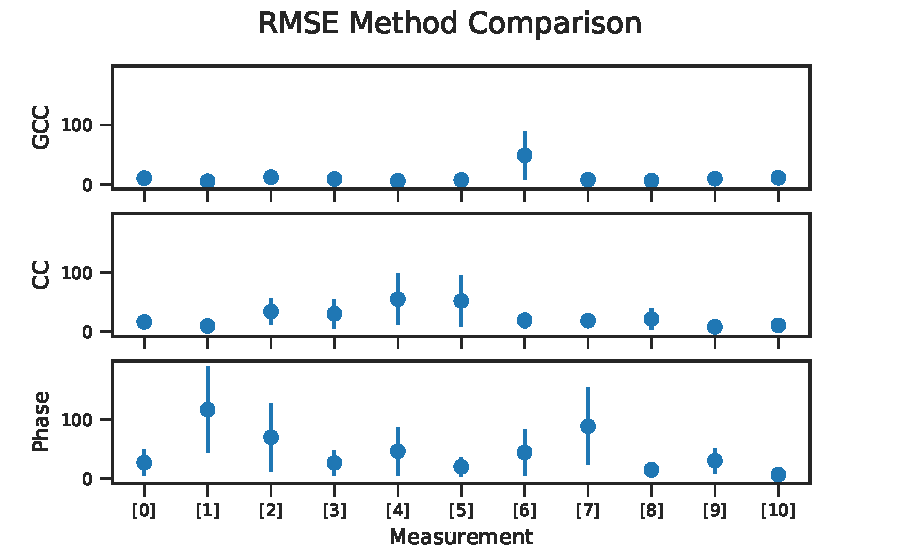
\includegraphics[]{figures/evaluation/compare_rmse}
	\caption{Angular RMSE and standard error of robot results per
		measurement of \cref{subsec:04_labMeasurements}.}
	\label{fig:04_compareRmse}
\end{figure}
% -------------------------------------------------------------

\subsection{Conclusion}
\label{subsec:04_tdoaConclusion}

The results in \Cref{subsec:04_singleRobotAngleError} show
that the \ac{GCC-PHAT} algorithm performs best according to the
laboratory-measurements.
Not only the errors are smallest, but also the low standard deviation
displays that the robots agree on the \ac{WSDE} and little outliers exist.
Also in regard to the multi-agent Bayesian updating filter, unified
results of the stand-alone robots are beneficial.
Another advantage of the \ac{GCC-PHAT} method is the presence of
an indication regarding the certainty of the measurement.
Interpreting the \ac{PSNR} as such, it can be used to detect outliers
or consider results with small \ac{PSNR} less.

Regarding the computational effort, the phase difference method
with static reference frequencies for \ac{TDOA} estimation
accomplishes lowest demand.